% kapitel2.tex
\chapter{Analyse von RAD-Seq-Daten} \label{chapter:kap2}
\section{Problemstellung} \label{sec:probl}

Ausgangsmaterial für RAD-Seq-Analysen sind die Reads aus in der Regel gepoolten Probengemischen mehrerer Individuen. Durch entsprechende Barcodemarkierungen können die Reads den einzelnen Individuen zugeordnet werden. Durch die Verwendung gepoolter Probengemischen ist das Verfahren kostengünstiger und zeitsparender als die meisten anderen NGS-Verfahren. Die Reads stammen aus dem gesamten Genom, wobei sie nur kleinere Sequenzabschnitte zwischen den Schnittstellen der Restriktionsenzyme repräsentieren und damit nicht das gesamte Genom abbilden. Ein deutlicher Vorteil des Verfahrens besteht darin, die Reads ohne Kenntnis eines Referenzgenoms möglichen Loci zuordnen zu können. Auch die Loci und ihre Sequenz sind somit anfangs unbekannt und werden erst durch die Analyse ermittelt.\\

Das RAD-Sequencing-Verfahren bedingt, dass durch die Restriktionsenzyme die DNA nur in innerhalb spezifischer Sequenzen geschnitten wird und dass durch PCR und Sequenzierung mehrere Reads erzeugt werden, die jeweils vom gleichen Locus stammen. Das hier implementierte Tool NodeRAD stellt einen Prototypen dar, der im Gegensatz zu derzeit etablierten RADSeq-Tools, wie beispielsweise dem Tool Stacks \cite{catchen_2013}, mit Hilfe von nur zwei Parametern diese Zuordnung realisiert. Das Clustering der Reads sowie die Identifizierung und Locizuordnung sollen dabei unter Berücksichtigung der Ploidie ohne weiteres Vorwissen allein auf Grundlage der Sequenzierfehlerrate und Heterozygotiewahrscheinlichkeit erfolgen. Die ermittelten Loci sollen für anschließende Diversitätsanalysen zur Verfügung stehen. 

\section{Formale Definition der Problemstellung} \label{sec:formal}

Gegeben sei eine Menge von Reads eines Individuums $ D = (s_{1}, \dots , s_{m}) \in \{A,\,C,\,G,\,T,\}^{k^m}$ mit der Readlänge $k$. In den Reads sind zudem für jede Base Informationen zur Qualität der Sequenzierung $ Q = (q_{1}, \dots , q_{m}) \in {[0,\,1]}^{k^m}$ enthalten. Weiterhin seien für Substitutionen, Insertionen und Deletionen die Heterozygotiewahrscheinlichkeit $\eta = (\eta_{sub},\, \eta_{ins},\, \eta_{del}) $ und für Indels die Sequenzierfehlerrate $\epsilon=(\epsilon_{ins},\, \epsilon_{del})$ gegeben. Ebenso ist die Ploidie $\phi$ des untersuchten Organismus bekannt. In der vorliegenden Arbeit wird im Model und beim implementierten Prototypen ein diploider Chromosomensatz vorausgesetzt, für höherploide Organismen ist eine Anpassung hinsichtlich des Sequenzalignments notwendig (siehe Kap. \ref{sec:ausblick}). \\

Ziel ist die Zuordnung der Reads zu den Loci unter Berücksichtigung von $\epsilon$ und $\eta$ sowie die Ausgabe der Menge der ermittelten Loci mit den Sequenzen der beteiligten Allele. Dabei soll die Menge von Loci gefunden werden, welche die beobachteten Reads am besten erklären kann, das heißt welche die höchste Wahrscheinlichkeit in Zusammenschau mit $\epsilon$ und $\eta$ besitzt. \\

\section{Lösungsansatz und Modell} \label{sec:solution}

Das Problem wird als gerichteter Graph betrachtet (siehe Kap. \ref{subsec:sol_graph}), dessen Knoten die einzelnen Reads beinhalten und dessen Kanten auf einem Sequenzalignment der Reads basieren. Für die Zuordnung der Reads soll das Problem in Teilprobleme aufgeteilt werden, für jedes Teilproblem wird dann eine Lösung ermittelt. Der Graph wird daher entsprechend seiner Zusammenhangskomponenten partitioniert. Die in einer Zusammenhangskomponente vorkommenden Sequenzen werden in Abhängigkeit von festgelegten Schwellwerten als Kandidatenallele betrachtet und jeweils mit sämtlichen Reads der Zusammenhangskomponente verglichen. Dabei sollen diejenigen Allele identifiziert werden, von denen die übrigen Reads der Komponente am wahrscheinlichsten durch Sequenzierfehler entstanden sind (Kap. \ref{subsec:sol_allele_lh}). Die Likelihoodberechnung hierfür wird durch die Basenqualität der Reads und Sequenzierfehlerrate bestimmt und erfolgt über alle Kombination möglicher Häufigkeitsverteilungen der Allele (Allele-Fractions). \\

Die Allele-Fraction mit der höchsten Likelihood $vaf_{max}$ soll anschließend für die Zuordnung der Loci verwendet werden (Kap. \ref{subsec:sol_loci_lh}). Hierfür wird die Likelihood für alle Loci-Kombinationen bestimmt, welche zu der ermittelten $vaf_{max}$ passen. Für die Berechnung der Likelihoods der Locizuordnung werden die Heterozygotiewahrscheinlichkeiten verwendet. Die Loci-Kombination mit der größten Likelihood wird schließlich als Lösung der betreffenden Zusammenhangskomponente ausgegeben (Kap. \ref{subsec:sol_vcf}).\\

Für jede Zusammenhangskomponente wird auf diese Weise also die wahrscheinlichste Lösung ermittelt, deren Komposition von Loci die beobachteten Reads innerhalb der Zusammenhangskomponente am besten erklären kann. Die Loci mit maximaler Likelihood aus allen Zusammenhangskomponenten werden schließlich durch NodeRAD im VCF-Format ausgegeben. Eine Übersicht der einzelnen Schritte des Workflows findet sich in \autoref{fig:workflow_all}.  \\
%https://texample.net/tikz/examples/labs-schema/
\usetikzlibrary{shadows,arrows}
% Layer des Diagramms
\pgfdeclarelayer{background}
\pgfdeclarelayer{foreground}
\pgfsetlayers{background,main,foreground}

% Eigenschaften der Blöcke 
\tikzstyle{blocktxt}=[draw, text width=6.0em, text centered,
minimum height=1.5em,drop shadow]
\tikzstyle{blockitem} = [blocktxt, fill=green!40, text width=8em, minimum width=10em,
minimum height=3em, rounded corners, drop shadow]
\tikzstyle{ioitem} = [blocktxt, fill=white, text width=8em, minimum width=10em,
minimum height=3em, rounded corners, drop shadow]
\tikzstyle{sectiontxt} = [above, text = black, text width=6em, text centered]
\tikzstyle{dashedline} = [draw, thick, color=black, -latex', dashed]
\tikzstyle{line} = [draw, thick, color=red, -latex']
\tikzstyle{ur}=[draw, text centered, minimum height=0.01em]

% Distanzen
\newcommand{\blockdist}{1.3}
\newcommand{\edgedist}{1.5}

\newcommand{\blockitem}[2]{node (p#1) [blockitem]
	{\textbf{\textit{#2}}}}

\newcommand{\ioitem}[2]{node (p#1) [ioitem]
	{\textbf{\textit{#2}}}}

% Eigenschaften der DNA-Abbildung
\newcommand{\bond}[3]{
	\draw[very thick, #1] (#3, 0) -- (#3, 0.35);
	\draw[very thick, densely dotted] (#3, 0.35) -- (#3, 0.65);
	\draw[very thick, #2] (#3, 0.65) -- (#3, 1);
}
% Hintergrundfeld
\newcommand{\background}[5]{%
	\begin{pgfonlayer}{background}
		% Hintergrundfeld obere linke Ecke
		\path (#1.west |- #2.north)+(-3.3,0.3) node (a1) {};
		% Hintergrundfeld untere rechte Ecke
		\path (#3.east |- #4.south)+(+0.5,-0.25) node (a2) {};
		% Hintergrundeigenschaften
		\path[fill=blue!20,rounded corners, draw=black]
		(a1) rectangle (a2);
		\path (a1.east |- a1.south) +(-3.0,-1.0) node (u1)[sectiontxt]
		{\textbf{\textit{#5}}};
\end{pgfonlayer}}

\newcommand{\out}[3]{%
	\path [dashedline] (#1.east) -- node [above]
	{\scriptsize Output: #2} (#3);}

\begin{figure}[]
	\begin{center}
		\begin{tikzpicture}[scale=0.66,transform shape]
			% https://github.com/PetarV-/TikZ/tree/master/DNA
			\path \ioitem {1}{Reads\\
				\begin{tikzpicture}[scale=0.6,transform shape]
				\bond{red}{blue}{0.1}
				\bond{red}{blue}{0.25}
				\bond{red}{blue}{0.4}
				\bond{blue}{red}{1.1}
				\bond{blue}{red}{1.25}
				\bond{blue}{red}{1.4}
				\bond{red}{blue}{2.1}
				\bond{red}{blue}{2.25}
				\bond{red}{blue}{2.4}
				\bond{blue}{red}{3.1}	
				\bond{blue}{red}{3.25}
				\bond{blue}{red}{3.4}
				\bond{red}{blue}{4.1}
				\bond{red}{blue}{4.25}
				\bond{red}{blue}{4.4}
				\braid[rotate=90,style strands={1}{red, very thick},style strands={2}{blue, very thick}] (tst) at (0, 0) s_1 s_1 s_1 s_1 ;
				\end{tikzpicture}
			};
			\path (p1.south)+(-2.5,-2.0) \blockitem{2}{Adapter trimming};
			\path (p2.south)+(2.5,-1.2) \blockitem{3}{Quality control};
			\path (p3.south)+(-2.5,-1.2) \blockitem{5}{Sequence alignment};
			\path (p3.west)+(4.75,-3.8) \blockitem{4}{Build graph};
			\path (p3.east)+(+9.8, 0.0) node (ur1)[ur] {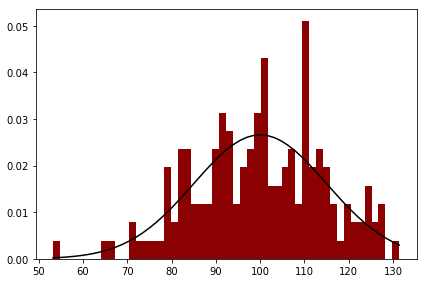
\includegraphics[width=2.0cm]{bilder/qc_reports_icon_5.png}};
			\path (p4.south)+(0.0,-1.5) \blockitem{6}{Connected components};
			\path (p4.east)+(+7.0,0) node (ur2)[ur] {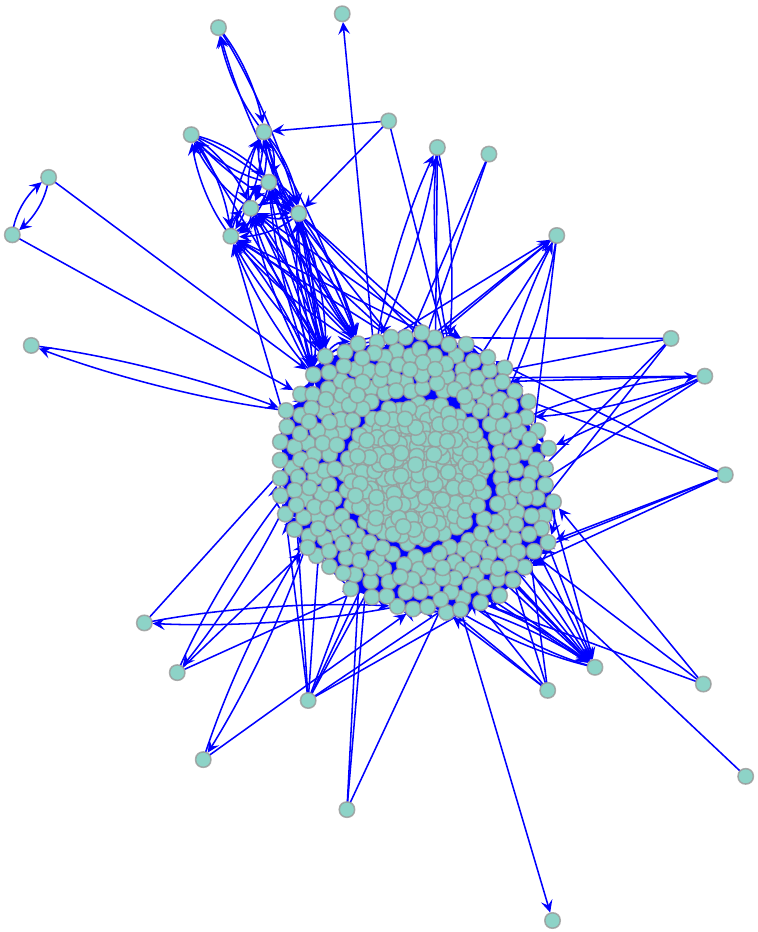
\includegraphics[width=2.0cm]{bilder/big_components_3.png}};
			\path (p6.south)+(-5.5,-1.4) \blockitem{7}{Allele \\combinations};
			\path (p6.south)+(0.0,-1.4) \blockitem{8}{Candidate Alleles};
			\path (p6.east)+(+6.5,0) node (ur3)[ur] {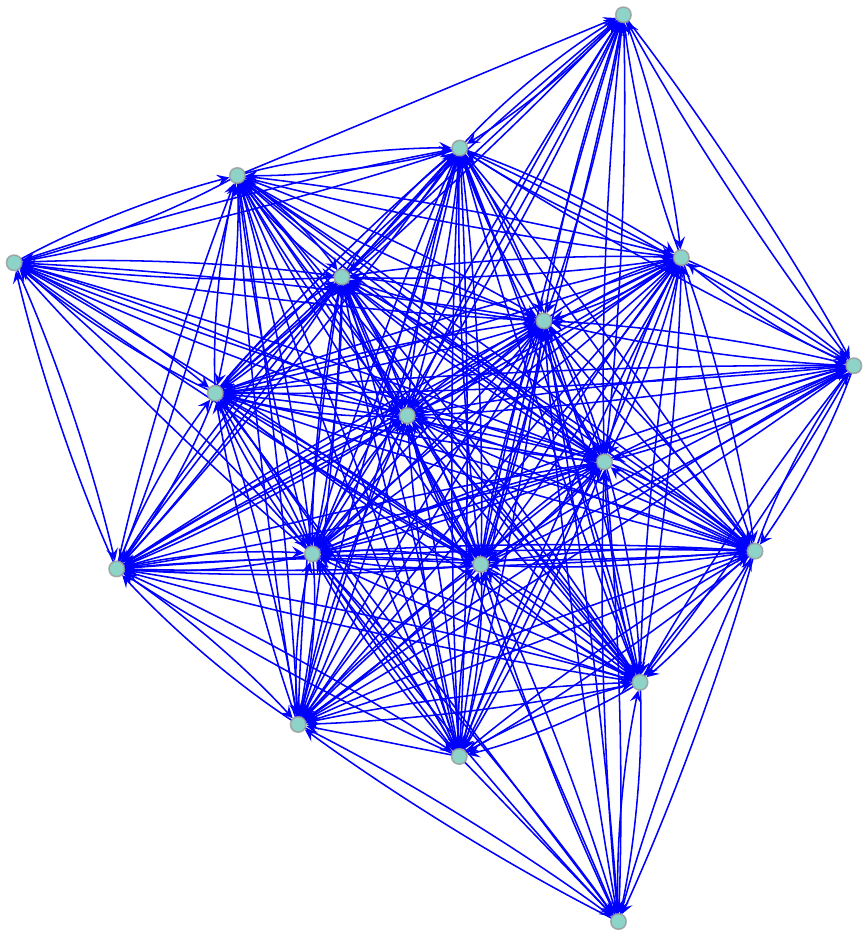
\includegraphics[width=1.0cm]{bilder/small_components_2.png}};				
			\path (p7.south)+(0.0,-3.87) \blockitem{9}{Allele fractions};
			\path (p8.south)+(0.0,-1.5)	\blockitem{10}{Likelihood of alleles given one read};
			\path (p9.south)+(0.0,-6.83) \blockitem{11}{Indicator constrait};
			\path (p10.south)+(0.0,-1.5) \blockitem{12}{Likelihood of allele fractions given one read};
			\path (p11.south)+(0.0,-1.5) \blockitem{13}{Loci \\combinations};
			\path (p12.south)+(0.0,-1.5) \blockitem{14}{Likelihood of allele fractions given all reads};
			\path (p14.south)+(0.0,-1.5) \blockitem{15}{Maximum likelihood allele fractions};
			\path (p15.south)+(0.0,-1.7) \blockitem{16}{Likelihood of an allele given another allele};
			\path (p16.south)+(0.0,-1.8) \blockitem{17}{Likelihood of loci given alleles and fractions}; 
			\path (p17.south)+(0.0,-1.3) \blockitem{18}{Maximum likelihood loci};
			\path (p18.south)+(0.0,-1.7) \ioitem{19}{VCF \\ 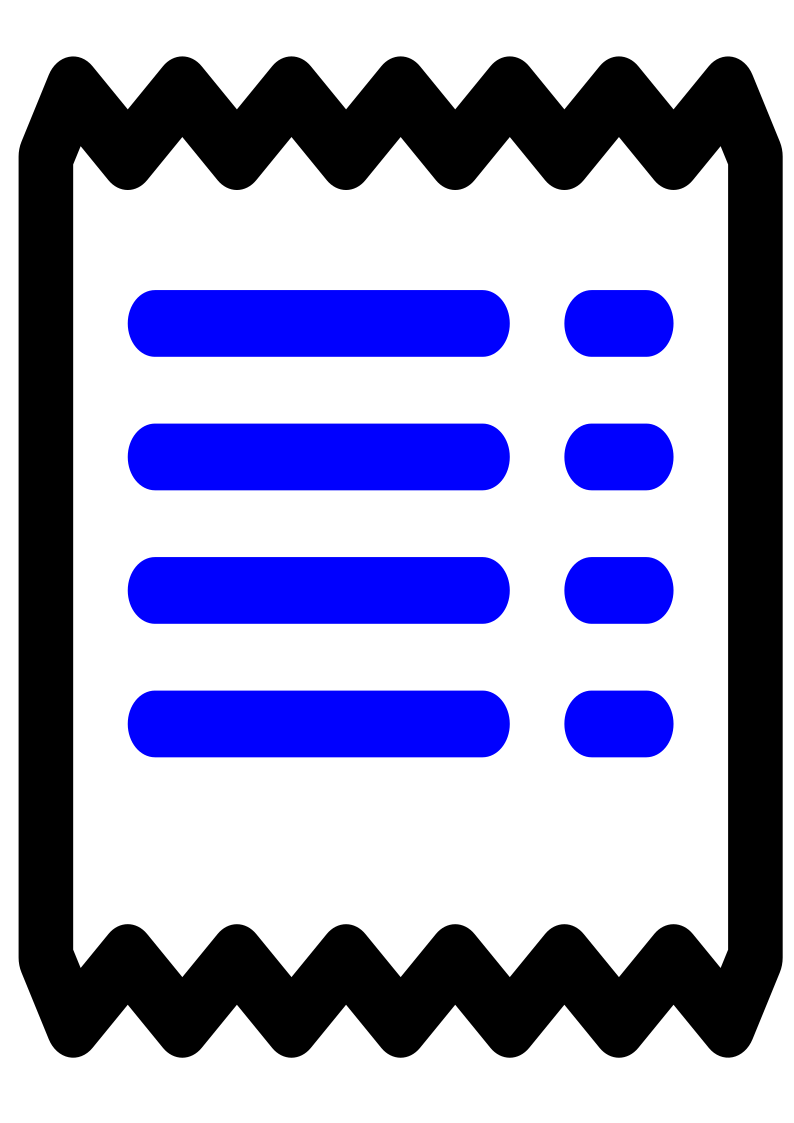
\includegraphics[width=0.9cm]{bilder/list_icon_2.png}\hspace{0.1cm}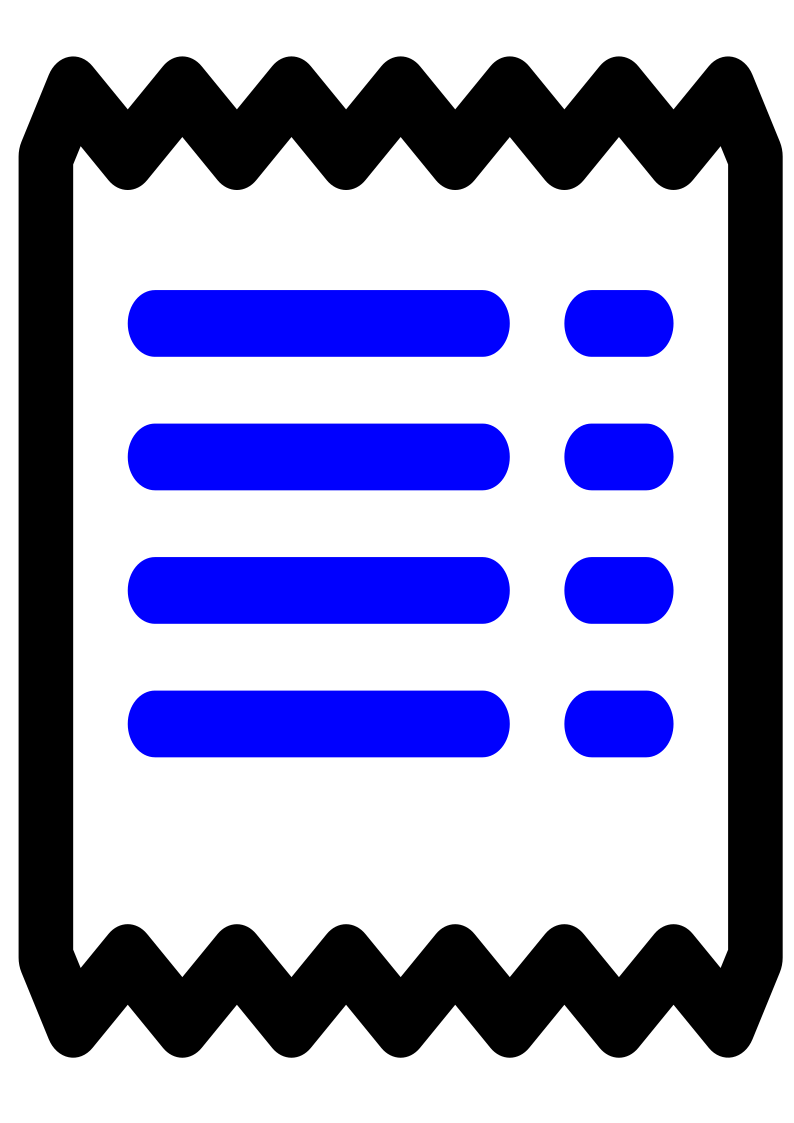
\includegraphics[width=0.9cm]{bilder/list_icon_2.png}\hspace{0.1cm}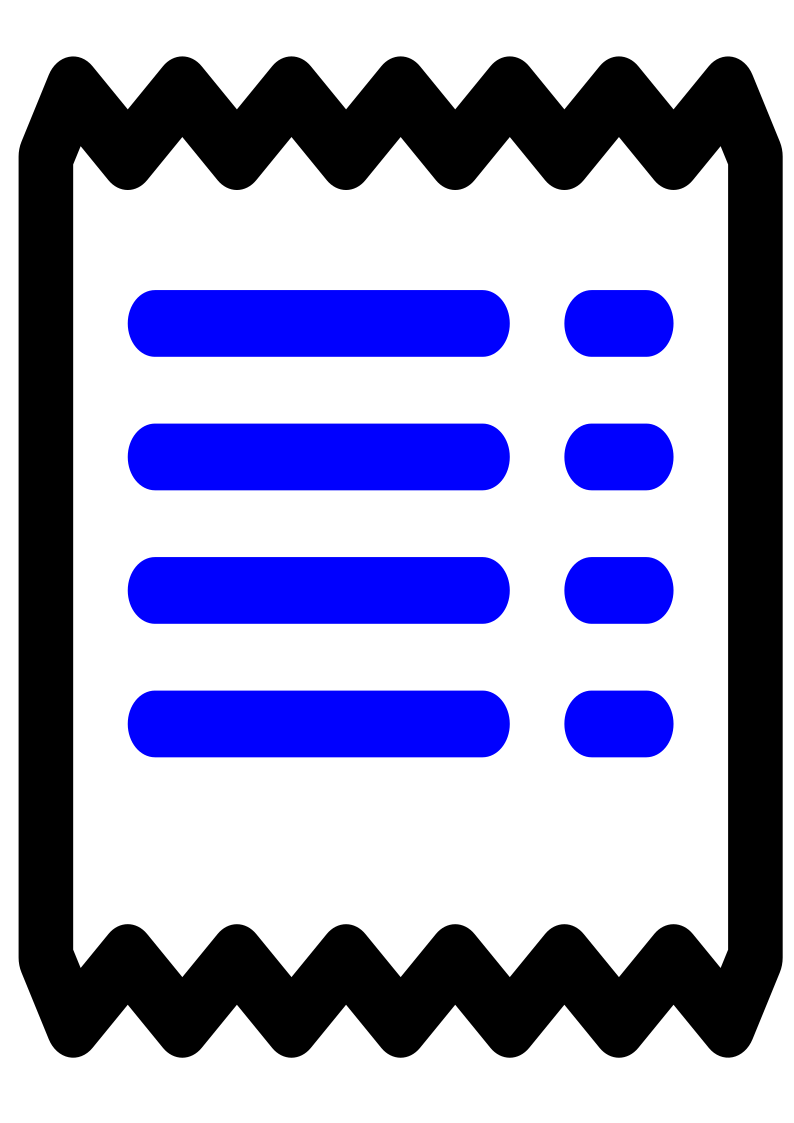
\includegraphics[width=0.9cm]{bilder/list_icon_2.png}};
			
			% Pfeile
			\path [line] (p1.south) -- +(0.0,-0.5) -- +(-2.5,-0.5) -- node [above, midway] {} (p2);
			\path [line] (p1.south) -- +(0.0,-0.5) -- +(+2.83,-0.5) -- node [above, midway] {} (p4);
			\path [line] (p2.south) -- node [above] {} (p3) ;
			\path [line] (p3.south) -- node [above] {} (p5) ;		
			\path [line] (p5.south) -- +(0.0,-1.415) -- node [above, midway] {} (p4.west);		
			\path [line] (p4.south) --node [above] {} (p6);
			\path [line] (p6.south) -- node [above] {} (p8);
			\path [line] (p8.south) -- node [above] {} (p10) ;	
			\path [line] (p10.south) -- node [above] {} (p12) ;	
			\path [line] (p12.south) -- node [above] {} (p14) ;		
			\path [line] (p14.south) -- node [above, midway] {} (p15);
			\path [line] (p15.south) -- node [above] {} (p16) ;     
			\path [line] (p16.south) -- node [above] {} (p17) ;
			\path [line] (p17.south) -- node [above] {} (p18) ;
			\path [line] (p18.south) -- node [above] {} (p19) ;		
			\path [line] (p19.south) -- +(0.0,-0.5) -- +(-8.8,-0.5) -- +(-8.8,26.327) -- node [above] {} (p5.west) ;
			
			\out{p3}{Reports (MultiQC, FastQC)}{ur1}
			\out{p4}{Graph, XML, DOT}{ur2}
			\out{p6}{Subgraphes, XML, DOT}{ur3}
			
			\path [dashedline] (p8.west) -- node [left] {} (p7);
			\path [dashedline] (p7.south) -- node [above] {} (p9) ;
			\path [dashedline] (p9.east) -- node [left] {} (p12.west);
			\path [dashedline] (p9.south) -- node [left] {} (p11.north);
			\path [dashedline] (p11.east) -- node [left] {} (p16.west);
			\path [dashedline] (p13.north) -- node [left] {} (p11.south); 
			
			\background{p3}{p2}{p3}{p5}{Preprocessing}
			\background{p3}{p4}{p4}{p6}{Graph \\construction}
			\background{p3}{p8}{p4}{p15}{Allele Likelihood}
			\background{p3}{p16}{p4}{p18}{Loci Likelihood}
 		\end{tikzpicture}
		\caption{Übersicht der Prozesse des Workflows}
		\label{fig:workflow_all}
	\end{center}
\end{figure}

\subsection{Graph und Zusammenhangskomponenten} \label{subsec:sol_graph}

Im Preprocessing wird aus den Reads zunächst ein paarweises Sequenzalignment mit Hilfe des Tools Minimap2 erzeugt ~\cite{li_2018}. Hierbei werden alle Reads mit einander verglichen und bei ausreichender Ähnlichkeit ihrer Sequenzen einander zugeordnet. Zusätzlich werden durch Minimap2 die Edit-Distanzen zwischen den jeweils verglichenen Readsequenzen bestimmt. \\

Wie bereits einleitend erwähnt, wird das Problem schließlich als gerichteter Graph $G=(V, \, E)$ mit der Knotenmenge $V$ und der Kantenmenge $E$ betrachtet. Die Knoten repräsentieren dabei die einzelnen Reads. Entsprechend dem von Minimap2 erzeugtem Sequenzalignment werden die Knoten der Reads durch Kanten verbunden. Die Kanten des Graphen repräsentieren somit den Vergleich der Sequenzen der beiden angrenzenden Reads. Die Anzahl der Kanten kann zusätzlich durch die von Minimap2 bestimmten Edit-Distanzen reguliert werden. Diese soll über einen konfigurierbaren Schwellwert flexibel wählbar sein und ermöglicht ein zusätzliches Filtern der Kanten zugunsten von  Laufzeit und Effizienz. \\

Da aufgrund des Sequenzalignments nur Reads mit einander verbunden werden, deren Sequenzen eine gewisse Ähnlichkeit zu einander aufweisen und da die RAD-Sequencing-Daten für gewöhnlich mehrere Loci beinhalten, ist der Graph in der Regel nicht zusammenhängend. Dies ermöglicht eine Unterteilung des Gesamtproblems in kleinere Teilprobleme durch Betrachtung der einzelnen Zusammenhangskomponenten des Graphen. Für diese Teilprobleme wird dann nach Lösungen gesucht. Da sich die Konstellation der Zusammenhangskomponenten direkt aus dem Sequenzalignment ergibt, sind die so entstandenen Cluster nicht notwendiger Weise nur einem einzigen Locus zuzuordnen. Vielmehr können die einzelnen Zusammenhangskomponenten auch jeweils mehrere Loci beinhalten. \\

\subsection{Approximation von PairHMM mittels Minimap2-Alignments} \label{subsec:phmm_minimap}

Wie bereits erwähnt, werden die Kanten des Graphen durch das Sequenzalignment repräsentiert. Dabei führt Minimap2 einen paarweisen Readvergleich anhand der DNA-Sequenzen der Reads durch. Die Sequenz jedes Reads (Querysequenz) wird mit jeder Sequenz der übrigen Reads (Referenzsequenz) verglichen. Reads mit hoher Ähnlichkeit zueinander werden in das Alignment aufgenommen. Das Ergebnis ist ein Mapping derjenigen Reads, die eine hohe Wahrscheinlichkeit besitzen, durch Sequenzierfehler, Variationen oder Mutationen aus einem gemeinsamen Allel hervorgegangen zu sein. Somit basieren die Kanten des Graphen auf den Wahrscheinlichkeiten des Sequenzalignments. \\

Das zugrundeliegende Modell ist hierbei ein vollständiger gerichteter Graph dessen Kantengewichte durch den paarweisen Sequenzvergleich eines pair Hidden Markov Models (pairHMM)~\cite{durbin_1998} errechnet werden. Das beobachtete Ergebnis der Referenzsequenz wird dabei durch Abfolgen von Mismatch-, Insertions und Deletions-Operationen der Querysequenz erklärt. Jede dieser Operationen stellt einen Zustand dar, der Übergang zwischen den Zuständen wird über Wahrscheinlichkeiten abgebildet. Die Zustände selbst sind allerdings nicht direkt beobachtbar. Die möglichen Kombinationen von Zustandsübergängen, die zum beobachteten Ergebnis der Referenzsequenz führen, können aber errechnet und als Matrix dargestellt werden. In der Matrix kann dann der wahrscheinlichste Pfad ermittelt werden. Hierfür muss gelten, dass auf diesem Pfad das Produkt über die Zustandsübergangswahrscheinlichkeiten der Matrix maximal ist. Als Ergebnis erhält man somit die wahrscheinlichste Zustandssequenz, um die Querysequenz in die Referezsequenz zu transformieren.\\

\noindent======================= draft =======================\\


 ergibt sich dabei aus dem Produkt der Zustandsübergangswahrscheinlichkeiten. kann aber die wahrscheinl Als Resultat entsteht eine Matrix mit den
Daher soll im vorliegenden Modell das Sequenzalignment durch Minimap2 als Approximation des zugrundeliegenden PairHMM betrachtet werden, welches

stellt dabei eine Approximation des pair Hidden Markov Models zum paarweisen Readvergleich dar (siehe Kap. \ref{subsec:phmm_minimap}). 
Grundlage für die Berechnung der Likelihoods der Kandidatenallele und der Loci ist das durch Minimap2 ermittelte Sequenzalignment. Minimap2 berechnet hier die

Dieses repräsentiert einen Pfad im der  pairHMM-Matrix, und zwar den Wahrscheinlichsten Pfad. Dieser dominiert ohnehin die Wahrscheinlichkeit die das pairHMM berechnen würde. Daher kannst du auch einfach nur die Wahrscheinlichkeit für diesen Pfad berechnen. Das ist ein Produkt über dem Alignment.  Dieses liefert die wird als Approximation als Approximation eine Pair hidden Markov Models ~\cite{durbin_1998} (PairHMM) betrachtet\\

~\cite{yoon_2009}
~\cite{knudsen_2003}
~\cite{durbin_1998}
-> Berücksichtigung der Basenqualität $q_{r}$ => Sequenzierfehler fließen mit geringerer likelihood in die weitere Berechnung ein -> werden weniger berücksichtigt und kommen seltener vor, z.T als noise entfernt-> loci likelihood wird mit den sequenzen mit seq-fehlern geringer sein -> seq-fehler gefiltert, da es nicht möglich ist eine  bessere lh für z.B. 3 Allele zu bekommen (von denen eines aber auf einem seq-fehler beruht), wenn es nur 2 tatsächliche Allele in einer komp gibt, d.h. lh für 2 Allele ist in diesem fall höher als für 3 -> loci likelihood enthält mutationen \\
paarweises Alignment aus Minimap2 als Teilproblem -> fast jede Beobachtung wird berücksichtigt\\
Bewertung/wslk ob ein read aus einem anderen read entstanden ist\\

%Die Berechnung der Likelihoods für die Vergleiche der Reads mit den Kandidatenallelen basiert auf dem in Kap. ~\ref{subsec:sol_phmm} beschriebenen pair Hidden Markov Model.
Hierbei repräsentiert das durch Minimap2 bestimmte Sequenzalignment bereits den wahrscheinlichsten Pfad durch die pairHMM-Matrix. Da dieser Pfad ohnehin die Wahrscheinlichkeit des pairHMM dominieren würde, wird zugunsten der Laufzeit direkt auf das Alignment von Minimap2 zurückgegriffen, um die Likelihoods zwischen den Readsequenzen zu bestimmen. Dabei werden die Sequenzierfehlerrate $ \epsilon $ und Basenqualität $ q_{query} $ durch die bereits zuvor ermittelte geschätzte Fehlerrate $ p_{query} $ berücksichtigt. Die Likelihood $ pairHMM_{\epsilon, q_{query}} \;(s_{ref}\;|\; s_{query}) $, dass der Queryread aus dem Referenzread allein durch Sequenzierfehler und Mutationen entstanden ist, errechnet sich schließlich aus dem Produkt der Likelihoods $ L_{i} $ für jede Base $ b $ an jeder Position $ i $ innerhalb der Sequenz $ s $ des Queryreads $ s_{query} $ im Vergleich zum Referenzread $ s_{ref} $.
 
\begin{equation} \label{eqn:2-5}
\tag{2-5}
pairHMM_{\epsilon, q_{query}} \;(s_{query}\;|\; s_{ref}) = \prod_{i=1}^{k}L_{i}
\end{equation}

!!!~\cite{kuhner_2014} seq-error

Jede Base $ b $ an Position $ i $ einer Readsequenz $ s $ der Länge $ k $ lässt sich also definieren als $ b \in \{\,b_{i}\in \{A,C,G,T\}^k\;,\; b_{i} \in s \;|\; i = 1, \dotsb, k \,\}$. Seien $ b_{i\,_{ref}} $ und $ b_{i\,_{query}} $ die Basen der Query- und der Referenzsequenzen an Position $ i $ einer Sequenz und $  p_{i\,_{query}} $ die geschätzte Fehlerrate von $ b_{i\,_{query}} $, die sich aus dem Phred Quality Score $ Q $ nach  \eqref{eqn:3-3} ergibt. Seien zudem $ m_{sub} $, $ m_{ins} $ und $ m_{del} $ die über die Konfigurationsdatei festgelegten Mutationsraten für Substitutionen, Insertionen und Deletionen. Dann errechnet sich die Likelihood $ L_{i} = Pr(b_{i\,_{ref}}\;|\; b_{i\,_{query}})$ an der Position $ i $ im Falle eine Matches unter Berücksichtigung der geschätzten Fehlerrate durch:
\begin{equation} \label{eqn:2-6}
\tag{2-6}
L_{i\,_{match}} = 1 - p_{i\,_{query}}
\end{equation}

Bei einem Mismatch dagegen müssen die Wahrscheinlichkeiten von Mutationen und Sequenzierfehlern berücksichtigt werden. Im Falle einer Mutation muss in die Wahrscheinlichkeit eines Matches auch die Mutationsrate des aufgetretenen Mismatches $ m_{rate} \in \{\,m_{sub},\,  m_{ins},\, m_{del}\,\} $ einbezogen werden:
\begin{equation} \label{eqn:2-7}
\tag{2-7}
L_{i\,_{mut}} = m_{rate}\; \cdotp \;(1 - p_{i\,_{query}})
\end{equation}

Die Wahrscheinlichkeit eines Sequenzierfehlers, also dass anstelle der sequenzierten Base tatsächlich eine der drei anderen Basen vorliegt, entspricht $ 1/3 $ der geschätzten Fehlerrate des Phred Quality Scores:
\begin{equation} \label{eqn:2-8}
\tag{2-8}
L_{i\,_{seqerr}} = \frac{1}{3} \; \cdotp \; p_{i\,_{query}}
\end{equation}

Aus \eqref{eqn:2-7} und \eqref{eqn:2-8} errechnet sich also die Likelihood bei einem Mismatch durch:
\begin{equation} \label{eqn:2-9}
\tag{2-9}
L_{i\,_{mismatch}} = (1-m_{rate}) \; \cdotp \; L_{seqerr} \; \cdotp \; L_{mut}
\end{equation}

Aus den Liklihoods von Matches \eqref{eqn:2-6} und Mismatches \eqref{eqn:2-7} kann somit schließlich nach \eqref{eqn:2-5} die Likelihood zwischen den Reads paarweise bestimmt werden.\\

------------
nur bei diploidie -> sonst multiples Sequenzalignment notwendig.

(vgl. Kap. ~\ref{subsec:sol_phmm}). Allerdings werden nun die Heterozygotiewahrscheinlichkeiten $\eta_{sub}$, $\eta_{ins}$ und $\eta_{del}$ der Grapheigenschaften zur Ermittlung der Likelihood nach Formel \eqref{eqn:2-20} genutzt.  \\

Das Sequenzalignment der Reads aus Minimap2 repräsentiert bereits den wahrscheinlichsten Pfad in der pairHMM-Matrix, so dass über diesen Pfad die Likelihoods der Allele (Kap. \ref{subsec:sol_allele_lh}) und der Loci (Kap. \ref{subsec:sol_loci_lh}) bestimmt werden können.

Dabei entspricht im Falle eines Mismatches die Likelihood der in der Konfigurationsdatei angegebenen Heterozygotiewahrscheinlichkeit $ \eta $ für die betreffende Mutationsart, also $ \eta_{sub} $ für Substitutionen , $ \eta_{ins} $ für Insertionen bzw. $ \eta_{del} $ Deletionen. Sei $i$ der Index der betreffenden Base innerhalb der betrachteten Allelsequenz und $ \eta_{rate} \in \{\,\eta_{sub},\, \eta_{ins},\, \eta_{del}\,\}$, dann berechnet sich bei einem Mismatch die Likelihood $L_{i}$ der Base nach Formel \eqref{eqn:2-10}.
\begin{equation} \label{eqn:2-10}
\tag{2-10}
L_{i\,_{mismatch}} = \eta_{rate}
\end{equation}

Im Falle eines Matches senkt die Möglichkeit eines Mismatches die Likelihood der betreffenden Base entsprechend um die Summe der Heterozygotiewahrscheinlichkeiten der genannten Mutationsarten (Formel \eqref{eqn:2-11}).
\begin{equation} \label{eqn:2-11}
\tag{2-11}
L_{i\,_{match}} = 1 - (\eta_{sub} + \eta_{ins} + \eta_{del})
\end{equation}

Die Likelihood $ Pr(T=a_{l_{j,2}} \, | \, S=a_{l_{j,1}}, \eta) $ des paarweisen Vergleichs der Allele $a_{l_{j,1}}$ und $a_{l_{j,2}}$ hinsichtlich der Zuordnung zu den Loci-Kombinationen errechnet sich schließlich aus dem Produkt der Wahrscheinlichkeiten der einzelnen Basen:
\begin{equation} \label{eqn:2-12}
\tag{2-12}
Pr(T=a_{l_{j,2}} \, | \, S=a_{l_{j,1}}, \eta) = pairHMM_{\eta}(a_{l_{j,1}}, a_{l_{j,2}}) = \prod_{i=1}^{k}L_{i}
\end{equation}

\subsection{Allele-Fractions mit maximaler Likelihood} \label{subsec:sol_allele_lh}

Um die Allele zu identifizieren, von denen die beobachteten Reads einer Zusammenhangskomponente am wahrscheinlichsten stammen, muss zunächst die Menge der Kandidatenallele $A=(a_{1}, \dots, a_{n}) \in \{A,\,C,\,G,\,T,\}^{k^n}$ bestimmt werden. Bei größeren Clustern ist davon auszugehen, dass die Sequenzen solcher Kandidatenallele mehrfach in den Reads auftauchen. Um den Aufwand der Likelihoodberechnung bei größeren Cluster anpassen zu können, soll es möglich sein, selten auftretende Sequenzen herauszufiltern. Dies geschieht über zwei Grenzwerte, welche die Mindestgröße des Clusters und die Mindesthäufigkeit von Kandidatenallelsequenzen festlegen. Durch sie werden ab einer bestimmten Clustergröße nur diejenigen Sequenzen in die Auswahl der Kandidatenallele aufgenommen, die mit einer bestimmten Häufigkeit im Cluster vorkommen.\\

Anschließend wird die Wahrscheinlichkeit bestimmt, dass ein Read mit der Readsequenz $s_{r}$ und mit der Fehlerrate $\epsilon$ tatsächlich von einem bestimmten Allel stammt. Die Fehlerrate $\epsilon$ ergibt sich dabei aus der Qualität der einzelnen Basen eines Reads. Jede Base der Sequenz des Source-Knotens wird mit der Sequenz des Target-Knotens verglichen. Bei einem sogenannten Mismatch unterscheiden sich die verglichenen Basen durch Substitutionen, Insertionen oder Deletionen. Im Falle eines Matches sind beide Basen identisch. Bei einem Match ergibt sich die Wahrscheinlichkeit $L_{match}$, dass es sich dabei im Source-Knoten tatsächlich um die korrekte Base handelt allein aus der Fehlerrate:
\begin{equation} \label{eqn:2-13}
\tag{2-13}
L_{match} = 1 - \epsilon
\end{equation}

Bei einem Mismatch $L_{mismatch}$ müssen die Wahrscheinlichkeiten für Sequenzierfehler $L_{sequerr}$ (vgl. Formel \eqref{eqn:2-8}) und Mutationen $L_{mut}$ (vgl. Formel \eqref{eqn:2-7}) sowie die Mutationsrate selbst $m_{rate}$ mit einbezogen werden: 
\begin{equation} \label{eqn:2-14}
\tag{2-14}
L_{mismatch} = (1 - m_{rate}) \, \cdotp L_{sequerr} \, \cdotp L_{mut}
\end{equation}

Die genaue Berechnung der Likelihood der einzelnen Basen wird an späterer Stelle in Kap. \ref{subsec:edges} ausführlicher besprochen. Das Produkt aller Wahrscheinlichkeiten der einzelnen Basen ergibt schließlich die Likelihood für den paarweisen Vergleich zweier Reads im Sinne des pairHMM. Bei paarweisen Vergleich eines Allels $a_{i} \in A $ mit einem Read mit der Sequenz $s_{r}$ lässt sich die Likelihoodberechnung also wie folgt formulieren:
\begin{equation} \label{eqn:2-15}
\tag{2-15}
Pr(T=s_{r} \, | \, S=a_{i}, \epsilon) = pairHMM_{\epsilon,q_{r}}(a_{i}, s_{r})
\end{equation}


\noindent======================= draft =======================\\

\noindent0. noise nicht als Kandidaten-Allele -> liste lexicogra. sortierter Allele\\

\noindent1. lh zwischen 1 read und 1 allel; likelihood im pair: Wslk, dasss von 1 bestimmten Allel $a_{i}$ mit Fehlerrate $\epsilon$ tatsächlich die readsequenz $s_{r}$ stammt \\
$s_{r}$ Sequenz von Read $r$, $q_{r}$ Basenqualität aller Basen von Read $r$, $a_{i}$ Allel $i$ aus der Menge der Kandidatenallele $A=(a_{1},\dots, a_{n})$ mit Anzahl $n$ und $\epsilon$ Sequenzierfehlerrate
\begin{equation} \label{eqn:2-16}
\tag{2-16}
Pr(T=s_{r} \, | \, S=a_{i}, \epsilon) = pairHMM_{\epsilon,q_{r}}(a_{i}, s_{r})
\end{equation}

\noindent2. Info über alle vafs aller Kandidatenallele für 1 read; Zusammenhangskomponenten kann auch >1 locus enthalten -> Fractions finden in der möglichen Menge von loci \\
Berechnung der Wslk, einen Read zu beobachten anhand der gegebenen Allele-Fraktion\\
die Wslk der Fraktion $\Theta_{i}$ muss sich aus den tatsächlichen Beobachtungen ergeben => Urnenmodell (entspricht binominal modell)\\
Urnenmodell: bsp. 2 farben in unterschiedl. Menge -> Wslk, wenn n Kugeln gezogen werden, dass dabei jeweils genau 50\% von jeder Farbe gezogen wurden (Binomial Formel), Anzahl der roten Kugeln P (Erfolgswslk) $\Theta_{i}$ und  > 2 Farben => Mulitnomialverteilung $\Theta_{i}$ + individuellen Verteilung $Pr$: $\Theta_{i} * Pr$
es gilt $\sum \Theta_{i} = 1$ => die mögliche Zuordnung entspricht der Häufigkeit die gezogen wurde $\Theta_{i}$ \\
Wslk. $ s_{r} $ zu beobachten unter der gegebenen Verteilung aus den Fraktionen; Wslk read zu sehen gegeben das Allel, nur ausgehend von Sequenzierfehlern \\
$\Theta=\theta_{1},\dots,\theta_{n}) \in [0,1]^n $ sind Allel-Fraktionen, $n$ ist Anzahl der Allele \\
\begin{equation} \label{eqn:2-17}
\tag{2-17}
Pr(s_{r} \, | \, \Theta=\theta_{1},\dots,\theta_{n}) = \sum_{i=1}^{n}\theta_{i} \, \cdotp Pr(T=s_{r} \, | \, S=a_{i}, \epsilon)
\end{equation}
\noindent3. Für alle Reads: \\
1 read $s_{r}$ mit $n$ candidaten allelen -> $n$ mögliche Allele von denen $s_{r}$ stammen kann -> es wird für jedes der allele wslk berechnet, dass die allele aus $s_{r}$ entstanden sind\\
bsp. allel i hat frac 0.25, also 1/4 für i, allel i+1 mit 0.75 => zu 25\% allel i und zu 75\% allel i+1 -> über max lh wird bestimmt, wie die seq der allele zusammenpassen -> modellierung ähnlicher,  unsicherheit bei der zuordung der reads, wenn sie weder der dem eine noch dem anderen allel entstammen, z.b. bei 0.5/0.5 => Unsicherheit wird an schritt 3 weitergegeben \\
Produkt über alle reads für jede mögliche Kombination an fractions \\
max wählen innerhalb der conn. comp\\
insgesamt:\\
=> $\Theta$ berechnen -> max lh aus allel-fractions\\
=> alles was an Unterschieden vorkommt, kann nur ein Sequenzierfehler sein\\
$m$ ist Anzahl der Reads, $L \in \{l_{i} \in \mathds{N}_{\leq n}^\phi \, | \, i=1, \dots, g\}$ ist Menge der Loci, $D = (s_{1}, \dots, s_{m}) \in \{A,C, G, T\}^{k^m}$ ist Menge der Readsequenzen/der Reads,
\begin{equation} \label{eqn:2-18}
\tag{2-18}
L(\Theta=\theta_{1},\dots,\theta_{n} \, | \, D) = Pr(D \, | \, \Theta=\theta_{1},\dots,\theta_{n}) = \prod_{r=1}^{m}Pr (s_{r} \, | \, \Theta=\theta_{1},\dots,\theta_{n})
\end{equation}
für jede vaf wurde also liklihood über alle reads bestimmt -> Maximum 


\subsection{Locuszuordnung mit maximaler Likelihood} \label{subsec:sol_loci_lh}
connected comp in loci aufsplitten\\
Zuordnung zu loci, also welche genomischen loci stecken dahinter, wie werden die allele den loci zugeordnet -> max parximony, prinzip der einfachsen möglichen lösung \\
-> ploidy als eingabeparam -> zuordnung der candidaten allele zu loci\\
lh ausrechnen aus anzahl der allele und loci -> gerade die loci, die die seq. der reads am besten unter der geg. ploidy und heterozygotie erklären haben max lh
max\_lh\_vafs nur noch 1 Vektor\\
Zuordnung von cand-Allelen zu den loci => die beobachteten max\_lh\_allel\_fractionen müssen sie durch die gewählten loci erklären, z.B. 2 loci => 1.locus: allel 0, 0 homozyg, 2. locus allel 0, 2 heterozygot\\
-> bei z.B 3 Allelen sind min 2 Loci notwendig => min \# der loci, so dass alle ausgewählten allele passen -> diese menge muss gefunden werden und muss wieder max lh haben\\
unter der annahme der loci-verteilung muss bestimmt werden ob sinnvoll, d.h allel-vafs müssen sich zu 1 summieren -> indikator-funktion: wenn 1, dann gilt Pr(T|S), d.h. Wslk, dass sich aus S die seq T gebildet hat\\

indicator-function $z_{l} \in {[0,1]}$: wird 1, wenn anzahl des auftretens aller allele $A = (a_{1}, \dots, a_{n})$ in einer möglichen locus-verteilung $l = (l_{1}, \dots, l_{g \, \cdotp \phi})$ jeweils genau ihrer absoluten Häufigkeit aus der in Kap. \ref{subsec:sol_allele_lh} errechneten vaf mit maximaler Likelihood entspricht, also $\theta_{i} \, \cdotp g \, \cdotp \phi$ entsprechen, andernfalls gilt $ z_{l} = 0 $. Seien dabei  $\Theta=\theta_{1},\dots,\theta_{n}) \in [0,1]^n $ die vaf mit maximaler Likelihood, $ \phi $ die Ploidie und gilt für eine mögliche Locusverteilung $l$ außerdem $L \in \{l_{j} \in \mathds{N}_{\leq n}^\phi \, | \, j=1, \dots, g\}$, so lässt sich die Indikatorfunktion wie folgt definieren:
\begin{equation} \label{eqn:2-19}
\tag{2-19}
z_{l}=\prod_{i=1}^{n}1_{\sum_{j=1}^{g}\sum_{k=1}^{\phi}1_{l_{j,k}=i} = \theta_{i} \, \cdotp g \, \cdotp \phi}
\end{equation}

pHMM: Wslk, dass allel 2 $ a_{l_{j,2}} $ aus allel 1 $ a_{l_{j,1}} $ entstanden ist -> heterozygotie $\eta$ (in conf konfigurierbar) =>$ match = 1 - (het_{sub} + het_{del} + het_{ins}) $
\begin{equation} \label{eqn:2-20}
\tag{2-20}
Pr(T=a_{l_{j,2}} \, | \, S=a_{l_{j,1}}, \eta) = pairHMM_{\eta}(a_{l_{j,1}}, a_{l_{j,2}})
\end{equation}

Kombi von loci -> lh berechnen
\begin{equation} \label{eqn:2-21}
\tag{2-21}
Pr(\Theta,A \, | \, L=\{l_{j}\, |\, j=1,\dots,g\})=z_{l} \, \cdotp \prod_{j=1}^{g}Pr(T=a_{l_{j,2}} \, | \, S=a_{l_{j,1}})
\end{equation}

=> maximum der loci Likelihoods wählen
\subsection{Varianten und Genotyp} \label{subsec:sol_vcf}
mit den allelen $A = (a_{1}, \dots, a_{n})$ jedes locus $L \in \{l_{j} \in \mathds{N}_{\leq n}^\phi \, | \, j=1, \dots, g\}$, allelsequenz, genotyp\\
Menge von Loci, die die Beobachtungen erklären